\chapter{Detection Methodology}
\label{chap:ch3}

\par This chapter presents the detection methodology employed by the system developed in this dissertation. It begins with an overview of the analysis pipeline and the foundational techniques, i.e. static code analysis, AST-based source code inspection and code smell detection, then describes the construction and analysis of the interservice dependency graph and the composite health score computation. The chapter concludes with a detailed description algorithm for each individual anti-pattern.

\section{Detection Techniques}
\label{sec:detection-techniques}

\par This section outlines the techniques used for detecting architectural anti-patterns in microservice systems. Figure~\ref{fig:analysis-pipeline} provides an overview of the analysis pipeline, showing how source code is processed through multiple stages to produce anti-pattern detection results.

\begin{figure}
    \centering
    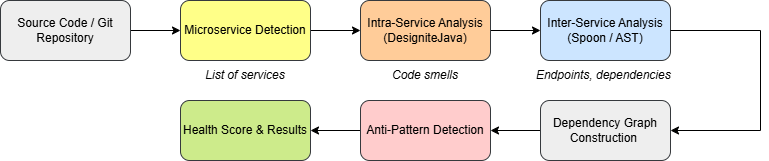
\includegraphics[scale=0.45]{figures/images/chapter3/analysis_pipeline.drawio.png}
    \caption{Overview of the anti-pattern detection pipeline. Source code is processed through microservice detection, intra-service and inter-service analysis, dependency graph construction, and anti-pattern detection, producing a health score and detailed results.}
    \label{fig:analysis-pipeline}
\end{figure}

\subsection{Static Code Analysis}
\label{subsec:static-analysis}

\par Static code analysis examines source code without executing it, allowing detection of structural issues, code smells, and architectural violations at the source level \cite{Chess2007}. In the context of microservices, static analysis can be applied at two levels. Intra-service analysis examines the internal structure of each microservice for code-level smells such as God Class, Long Method, Feature Envy, and Complex Method. The aforementioned smells serve as indicators of architectural problems at the service level. Inter-service analysis, on the other hand, examines the communication patterns, dependencies, and shared resources across microservices to detect architectural anti-patterns such as cyclic dependencies and shared databases.

\subsection{Abstract Syntax Tree Analysis with Spoon}
\label{subsec:spoon-analysis}

\par Spoon is an open-source library for analyzing, transforming and generating Java source code \cite{Pawlak2016}. It builds a fine-grained Abstract Syntax Tree (AST) that provides full access to all elements of the Java programming language, including annotations, method invocations and type references.

In this work, Spoon is used for inter-service analysis, specifically in three ways. Firstly, it detects REST controller endpoints by scanning for \texttt{@RestController}, \texttt{@GetMapping}, \texttt{@PostMapping} and other related annotations. Furthermore, it is used to identify inter-service communication by analyzing \texttt{@FeignClient} annotations, \texttt{@RestTemplate} method calls, and \texttt{@WebClient} builder patterns. Lastly, it extracts service metadata such as the number of endpoints, controller classes and API versioning information.

Beyond inter-service analysis, Spoon is also used for intra-service structural analysis. The God Service detector (Section~\ref{subsec:detect-god-service}) computes per-class metrics such as field count, public method count, import domain count, constructor parameter count and Tight Class Cohesion (TCC) directly from the AST. Similarly, the Chatty Service detector (Section~\ref{subsec:detect-chatty-service}) scans for interfaces and classes that exhibit chatty HTTP~client patterns by inspecting method annotations and verifying invocation target types.

The AST-based approach is more robust than regular expression-based scanning, as it understands the syntactic structure of the code and can resolve annotation attributes, method call chains and type hierarchies.

\subsection{Code Smell Detection with DesigniteJava}
\label{subsec:designite-analysis}

\par DesigniteJava is a static analysis tool that detects design smells, implementation smells and architecture smells in Java projects \cite{Sharma2018}. It analyzes Java source code and produces CSV reports categorizing detected smells by type, affected class and file location.

% The tool detects three categories of smells, summarized in Table~\ref{tab:code-smell-categories}.

In this dissertation, DesigniteJava is integrated as an external tool invoked as a subprocess. The analysis pipeline passes each detected microservice's source directory to DesigniteJava, parses the resulting CSV output files (\texttt{DesignSmells.csv}, \texttt{ImplementationSmells.csv}, \texttt{ArchitectureSmells.csv}), and stores the results in the application database. The God Class smell frequency per service is then used as a signal for god service detection (see Section~\ref{subsec:god-service}).

\begin{table}[htbp]
    \centering
    \footnotesize
    \begin{tabular}{|l|l|p{5.5cm}|l|}
        \hline
        \textbf{Category} & \textbf{Smell Name} & \textbf{Description} & \textbf{Severity} \\
        \hline\hline
        \multirow{4}{*}{Design} & God Class & Class with too many responsibilities & High \\
        \cline{2-4}
        & Feature Envy & Method more interested in other classes & High \\
        \cline{2-4}
        & Insufficient Modularization & Large, poorly modularized class & Medium \\
        \cline{2-4}
        & Unnecessary Abstraction & Abstraction without clear purpose & Low \\
        \hline
        \multirow{4}{*}{Implementation} & Long Method & Method with excessive length & Medium \\
        \cline{2-4}
        & Complex Method & Method with high cyclomatic complexity & Medium \\
        \cline{2-4}
        & Long Parameter List & Method with too many parameters & Medium \\
        \cline{2-4}
        & Magic Number & Unexplained numeric literals & Low \\
        \hline
        \multirow{3}{*}{Architecture} & Cyclic Dependency & Circular dependencies between packages & High \\
        \cline{2-4}
        & Unstable Dependency & Depending on less stable components & Medium \\
        \cline{2-4}
        & Hub-like Dependency & Class depended upon by many others & Medium \\
        \hline
    \end{tabular}
    \caption{Code smell categories detected by DesigniteJava, with their descriptions and severity mappings used in this work.}
    \label{tab:code-smell-categories}
\end{table}

\subsection{Dependency Graph Construction and Analysis}
\label{subsec:graph-analysis}

\par The dependency graph is a directed graph $G = (V, E)$ where each vertex $v \in V$ represents a microservice and each edge $e = (s, t) \in E$ represents a dependency from service $s$ to service $t$. Edges are annotated with metadata including the dependency type (REST synchronous, Feign client, messaging, etc.) and the call count.

\par A central challenge in dependency graph construction is resolving the target of an inter-service call to an actual microservice in the project. In real-world codebases, services are referenced by a variety of identifiers: directory names, \texttt{spring\-.application.name} values, \texttt{localhost:PORT} URLs, or Spring property placeholders injected via \texttt{@Value} annotations. To address this, the dependency graph builder employs a multi-strategy resolution pipeline.

\par The first step is a configuration pre-scan: before scanning source code, each service's \texttt{application.yml} or \texttt{application.properties} is parsed. The \texttt{spring\-.application.name} property is registered as an alias for the service directory name, and \texttt{server.port} values are recorded in a port-to-service mapping. Next, the pipeline performs \texttt{@Value} field resolution, in which fields annotated with Spring's \texttt{@Value} (e.g., \texttt{@Value("\$\{order\--service.url:http://localhost:8081\}")}) are pre-scanned using Spoon. Property placeholders are resolved against the service's configuration, falling back to default values when the property key is not found. Finally, a cascading target resolution strategy is applied: when a call target is extracted from a \texttt{@FeignClient} annotation, \texttt{RestTemplate} invocation, or \texttt{WebClient} call, it is matched to a microservice using three strategies applied in order, i.e. exact match against service names and registered aliases, port-based matching for \texttt{localhost:PORT}-style targets, and fuzzy substring matching with common suffix stripping (e.g., matching ''order'' to ''order-service''). For \texttt{@FeignClient} interfaces, each non-default, non-static method is registered as a separate call evidence entry, since each method corresponds to an individual HTTP request at runtime. This produces accurate per-method call counts that feed into chatty service detection.

Figure~\ref{fig:dependency-graph-example} shows an example dependency graph for a hypothetical microservice system. Each node represents a service, and edges are labeled with the dependency type and call count. The graph reveals a cycle between the Order, Inventory and Payment services as well as a potential ESB misuse pattern where the API Gateway mediates most communication.

\begin{figure}
    \centering
    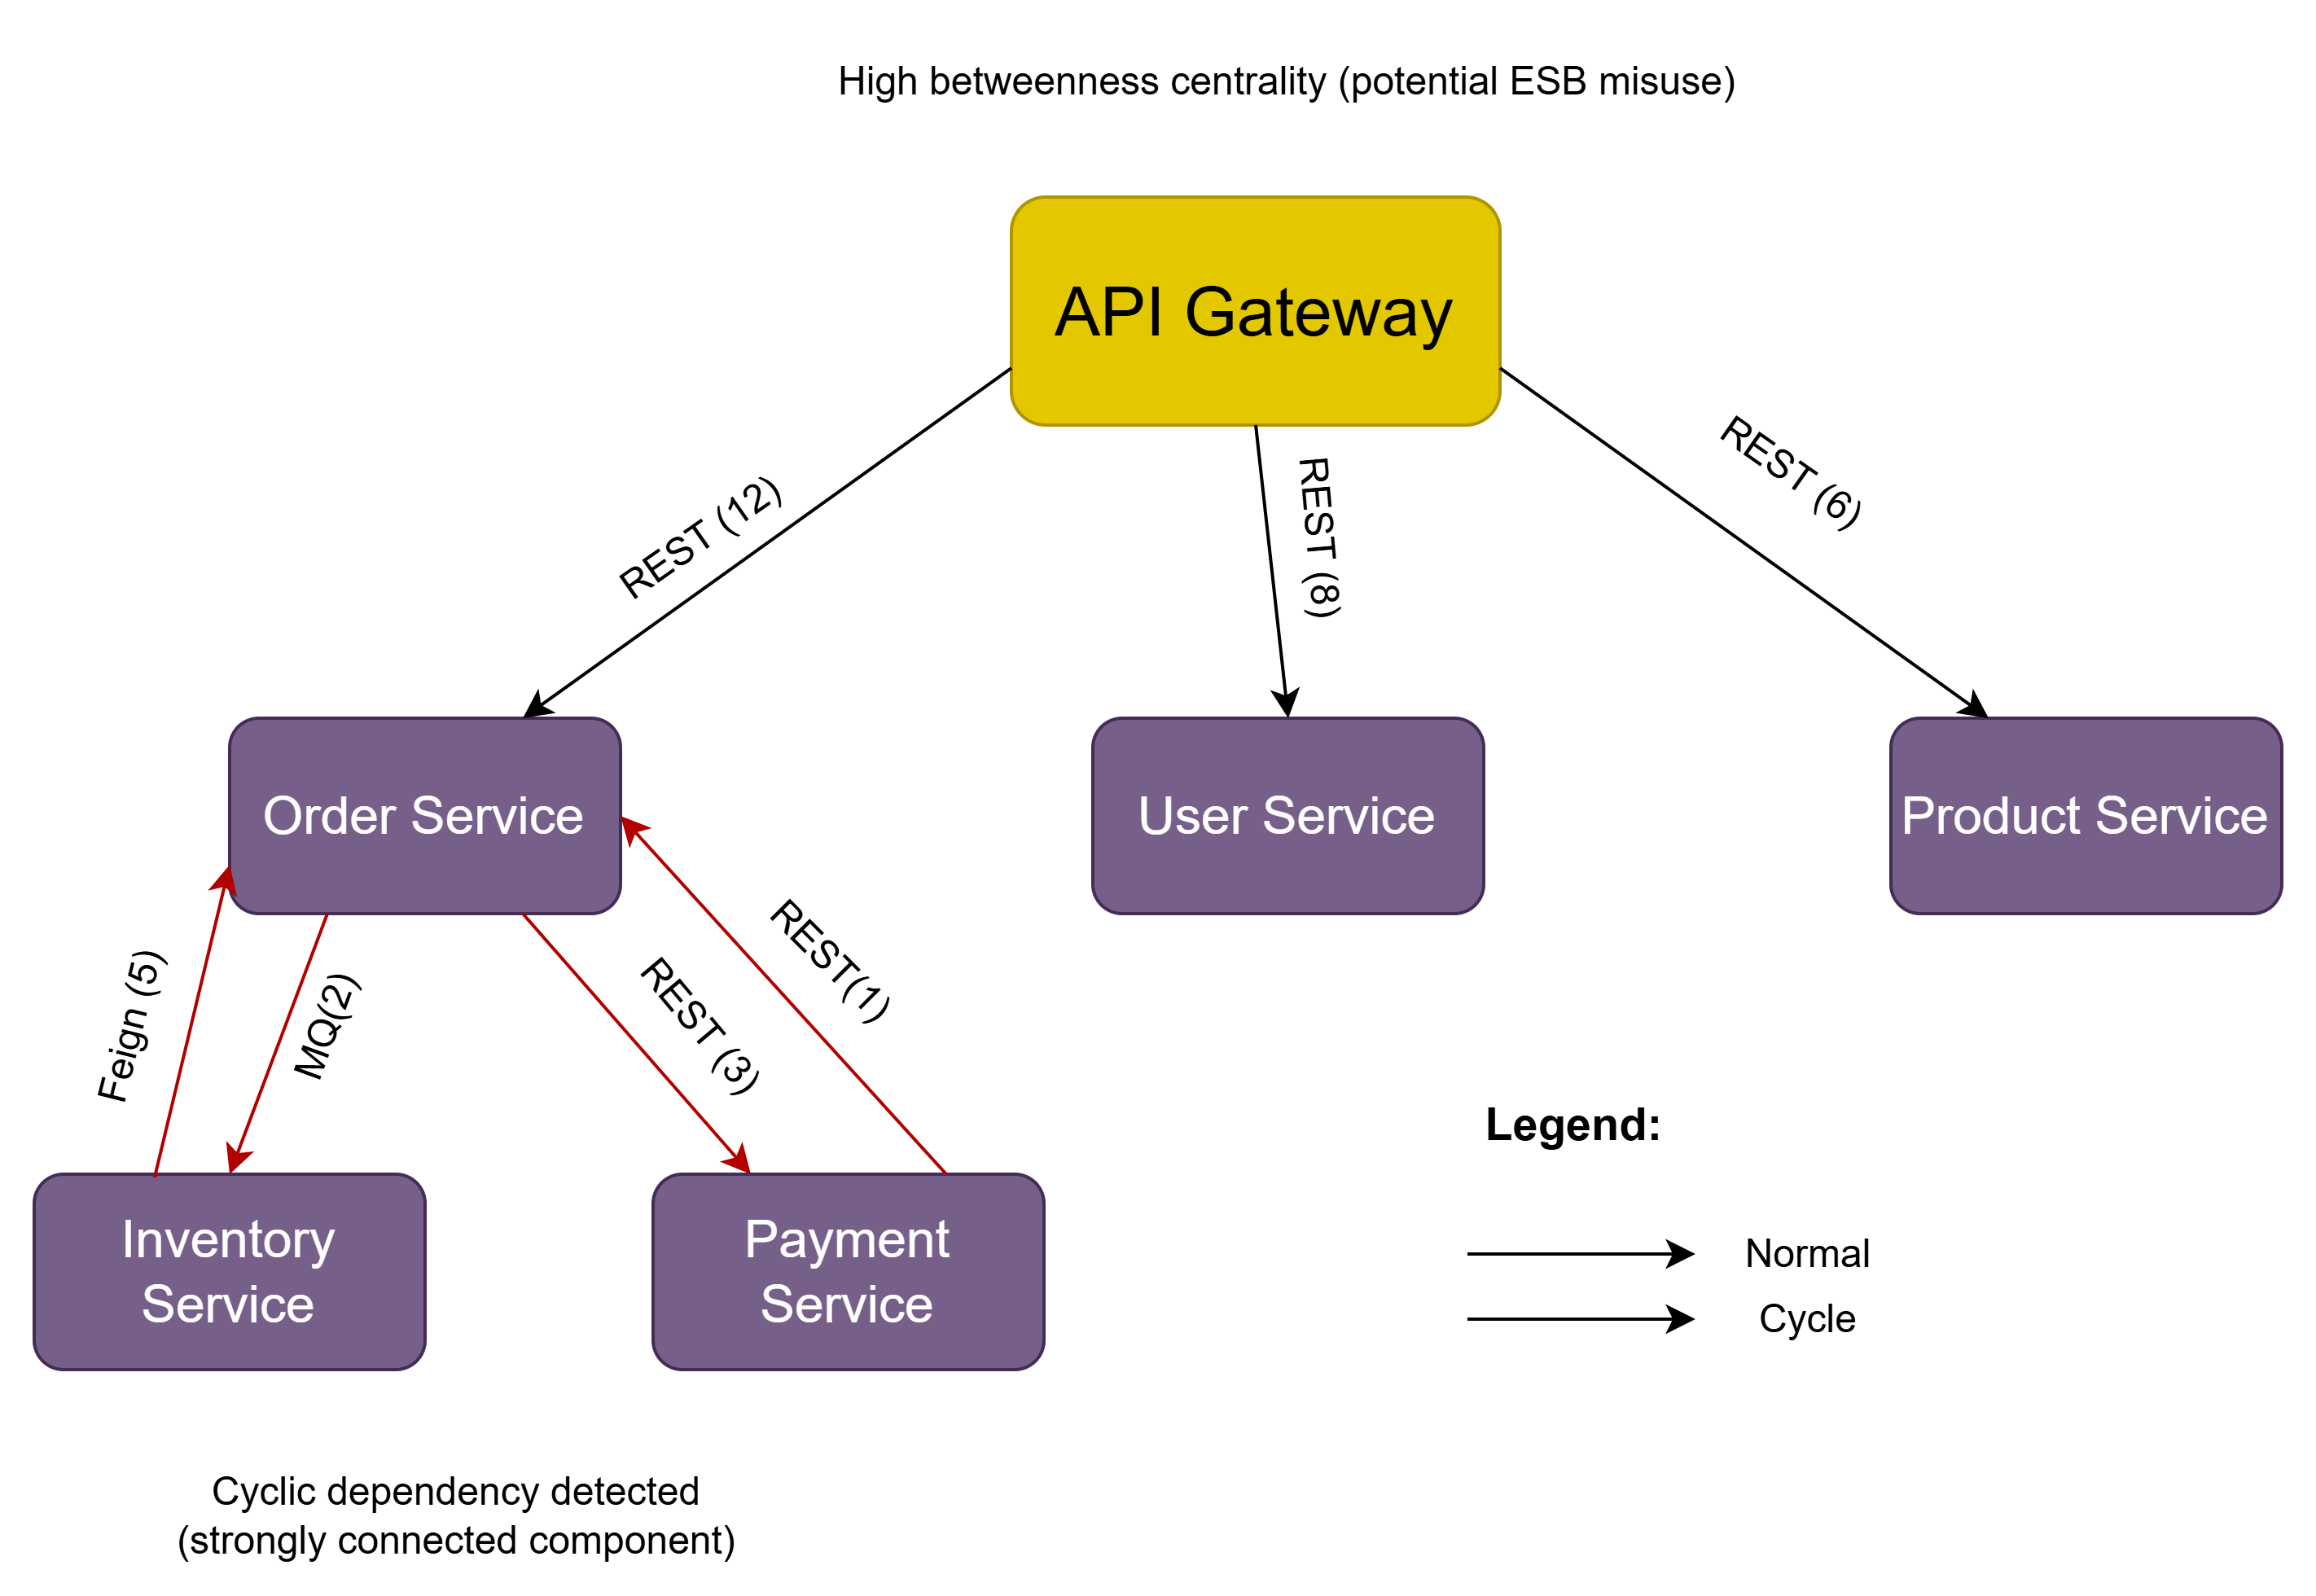
\includegraphics[scale=0.1]{figures/images/chapter3/dependency_graph_example.png}
    \caption{Example dependency graph for a microservice system. Nodes represent services, edges represent dependencies with type and call count annotations. The red dashed edges indicate a cyclic dependency. The API Gateway node exhibits high centrality, potentially indicating ESB misuse.}
    \label{fig:dependency-graph-example}
\end{figure}

\par Graph-based anti-pattern detection encompasses several analytical techniques. Cycle detection involves finding strongly connected components using Tarjan's algorithm to identify cyclic dependencies, while centrality analysis computes betweenness centrality to detect potential ESB misuse, where a single service mediates a disproportionate share of communication. Additionally, coupling metrics are evaluated by computing the coupling coefficient as the ratio of actual dependencies to possible dependencies.

\begin{equation}
    C = \frac{|E|}{|V| \times (|V| - 1)}
    \label{eq:coupling-coefficient}
\end{equation}

\noindent A high coupling coefficient suggests that the system may be a distributed monolith rather than a collection of loosely coupled services.

\subsection{Health Score Computation}
\label{subsec:health-score}

% TO-DO: go into a bit more depth maybe and/or revise this score

\par To provide an overall assessment of a system's architectural health, this dissertation computes a composite health score using a category-based decomposition. The total budget of 100~points is divided across four categories, each with an independent cap:

\begin{equation}
    H = S_{\mathrm{ap}} + S_{\mathrm{cq}} + S_{\mathrm{arch}} + S_{\mathrm{sz}}
    \label{eq:health-score}
\end{equation}

\noindent where each category score $S_i = \max(0,\; M_i - P_i)$, with $M_i$ the maximum budget and $P_i$ the total penalty for that category. The four categories and their budgets are described in the following paragraphs.

\par The first category, Anti-Patterns ($M_{\mathrm{ap}} = 40$), penalises each detected anti-pattern according to its severity (Table~\ref{tab:severity-weights}). The deduction per issue is 8~points for critical severity, 5 for high, 3 for medium, and 1 for low.

\par The second category, Code Quality ($M_{\mathrm{cq}} = 20$), captures the density of code smells reported by DesigniteJava. The penalty is computed on a logarithmic scale, $P_{\mathrm{cq}} = \min(20,\; \lfloor \ln(1 + n_{\mathrm{smells}}) \times 3.5 \rceil)$, which dampens the impact of very large smell counts while still penalising smell-heavy codebases.

\par The third category, Architecture ($M_{\mathrm{arch}} = 25$), assesses the structural quality of the dependency graph. The penalty is derived from the coupling coefficient, $\min(15,\; \lfloor c \times 15 \rceil)$ when $c > 0.1$, and the number of dependency cycles, $\min(10,\; 5 \times n_{\mathrm{cycles}})$.

\par The fourth category, Service Sizing ($M_{\mathrm{sz}} = 15$), evaluates the appropriateness of individual service granularity. Nano services incur a penalty of 3~points each (capped at~8) and god services incur 5~points each (capped at~10).


\par The final score is clamped to $[0, 100]$ and mapped to a letter grade: A~($\geq 90$), B~($\geq 80$), C~($\geq 65$), D~($\geq 50$), F~($< 50$). This category-based decomposition enables teams to identify which quality dimension contributes most to architectural debt and to track improvements per category over time.

Table~\ref{tab:severity-weights} details the severity levels, their corresponding penalty weights in the anti-pattern category, and examples of anti-patterns assigned to each level.

\begin{table}[htbp]
    \centering
    \footnotesize
    \begin{tabular}{|l|c|c|p{6.5cm}|}
        \hline
        \textbf{Severity} & \textbf{Weight} & \textbf{Penalty} & \textbf{Example Anti-Patterns} \\
        \hline\hline
        Critical & 4 & $-8$ per issue & Cyclic Dependency, Distributed Monolith \\
        \hline
        High & 3 & $-5$ per issue & Shared Database, God Service, Wrong Cuts, Chatty Service, ESB Misuse \\
        \hline
        Medium & 2 & $-3$ per issue & Nano Service, Hardcoded Endpoints, API Versioning Absence \\
        \hline
        Low & 1 & $-1$ per issue & --- \\
        \hline
    \end{tabular}
    \caption{Severity levels with their penalty deductions in the anti-pattern category of the health score computation (Equation~\ref{eq:health-score}).}
    \label{tab:severity-weights}
\end{table}

\section{Per-Anti-Pattern Detection Methodology}
\label{sec:per-anti-pattern-detection}

\par This section describes the detection algorithm for each anti-pattern targeted by this work. For each anti-pattern, the input data, detection logic, configurable thresholds, and evidence collection mechanism are presented. The definitions and motivations for each anti-pattern were introduced in Chapter~\ref{chap:ch2}; this section focuses on the \textit{how} of detection.

\subsection{Shared Database Detection}
\label{subsec:detect-shared-database}

\par The Shared Database detector operates by comparing the datasource connection URLs configured across all detected microservices. The algorithm proceeds in two phases.

In the first phase, the configuration files of each microservice are parsed to extract the datasource URL. For Spring Boot applications, the detector reads \texttt{application.yml}, \texttt{application.yaml}, or \texttt{application.properties} configuration files located in the \texttt{/resources} directory of each service. From YAML files, the nested property \texttt{spring.datasource.url} is extract using a recursive map traversal, whereas from properties files, the same key is read directly. Spring property placeholders with default values (e.g., \texttt{\$\{DB\_HOST:localhost\}}) are resolved to their defaults to enable meaningful comparison.

In the second phase, microservices are grouped by their resolved datasource URL. Any group containing more than one service indicates a shared database instance. Formally, let $\mathcal{S}$ denote the set of all microservices and $\mathit{dsUrl}$ denote the resolved datasource URL of service $s$. The detector reports a Shared Database anti-pattern for each equivalence class:

\begin{equation}
    \forall\, u \in \mathit{URLs} : \bigl|\{s \in \mathcal{S} : \mathit{dsUrl}(s) = u\}\bigr| > 1
    \label{eq:shared-db-detection}
\end{equation}

For each detected instance, the detector extracts a code snippet from the configuration file of each sharing service, highlighting the line containing the datasource declaration, for immediate evidence for remediation.

Algorithm~\ref{alg:shared-database} summarises the detection procedure.

\begin{algorithm}[htbp]
\caption{Shared Database Detection}\label{alg:shared-database}
\begin{algorithmic}[1]
    \Require Set of microservices $\mathcal{S}$, project root path $P$
    \Ensure Set of detected Shared Database anti-patterns
    \State $\text{urlMap} \gets \emptyset$ \Comment{Map: datasource URL $\to$ list of services}
    \For{each service $s \in \mathcal{S}$}
        \State $u \gets \Call{ParseDatasourceUrl}{P, s}$
        \If{$u \neq \texttt{null}$}
            \State $\text{urlMap}[u] \gets \text{urlMap}[u] \cup \{s\}$
        \EndIf
    \EndFor
    \State $\text{results} \gets \emptyset$
    \For{each $(u, \text{services}) \in \text{urlMap}$}
        \If{$|\text{services}| > 1$}
            \State $\text{snippets} \gets$ \Call{ReadDatasourceSnippets}{P, \text{services}}
            \State $\text{results} \gets \text{results} \cup \{\text{SharedDB}(u, \text{services}, \text{snippets})\}$
        \EndIf
    \EndFor
    \State \Return $\text{results}$
\end{algorithmic}
\end{algorithm}

\subsection{Cyclic Dependency Detection}
\label{subsec:detect-cyclic-dependency}

\par Cyclic dependency detection is performed on the directed dependency graph $G = (V, E)$ constructed in the inter-service analysis-phase (see Section~\ref{subsec:graph-analysis}). The detector applies Tarjan's algorithm for finding strongly connected components (SCCs) \cite{Tarjan1972}. Any SCC containing more than one vertex represents a dependency cycle among the corresponding services.

The algorithm operates in $O(|V| + |E|)$ time. It performs a depth-first traversal of the graph, maintaining for each vertex $v$ two values: $\text{index}(v)$, the order in which $v$ was visited and $\text{lowlink}(v)$, the smallest index reachable from $v$ through the DFS subtree and back edges. A vertex $v$ is the root of an SCC when $\text{lowlink}(v) = \text{index}(v)$, at which point all vertices on the stack above $v$ (inclusive) form the SCC.

Algorithm~\ref{alg:tarjan} presents the implementation of Tarjan's SCC algorithm as used in this work. The outer loop (lines 4--8) ensures all vertices are visited even in disconnected graphs.

\begin{algorithm}[htbp]
\caption{Tarjan's SCC Algorithm for Cycle Detection}\label{alg:tarjan}
\begin{algorithmic}[1]
    \Require Directed graph $G = (V, E)$
    \Ensure List of strongly connected components
    \State $\text{index} \gets 0$; $\text{stack} \gets \emptyset$; $\text{result} \gets \emptyset$
    \State $\text{idx}[v] \gets \text{undefined}$, $\text{low}[v] \gets \text{undefined}$ for all $v \in V$
    \State $\text{onStack}[v] \gets \texttt{false}$ for all $v \in V$
    \For{each $v \in V$}
        \If{$\text{idx}[v]$ is undefined}
            \State \Call{StrongConnect}{$v$}
        \EndIf
    \EndFor
    \State \Return $\text{result}$
    \Statex
    \Procedure{StrongConnect}{$v$}
        \State $\text{idx}[v] \gets \text{index}$; $\text{low}[v] \gets \text{index}$; $\text{index} \gets \text{index} + 1$
        \State Push $v$ onto stack; $\text{onStack}[v] \gets \texttt{true}$
        \For{each $(v, w) \in E$}
            \If{$\text{idx}[w]$ is undefined}
                \State \Call{StrongConnect}{$w$}
                \State $\text{low}[v] \gets \min(\text{low}[v], \text{low}[w])$
            \ElsIf{$\text{onStack}[w]$}
            \State $\text{low}[v] \gets \min(\text{low}[v], \text{idx}[w])$
            \EndIf
        \EndFor
        \If{$\text{low}[v] = \text{idx}[v]$}
            \State $\text{scc} \gets \emptyset$
            \Repeat
                \State Pop $w$ from stack; $\text{onStack}[w] \gets \texttt{false}$
                \State $\text{scc} \gets \text{scc} \cup \{w\}$
            \Until{$w = v$}
            \State $\text{result} \gets \text{result} \cup \{\text{scc}\}$
        \EndIf
    \EndProcedure
\end{algorithmic}
\end{algorithm}

For each SCC with $|\text{scc}| > 1$, the detector constructs a human-readable cycle description (e.g., ''Order Service $\to$ Payment Service $\to$ Order Service'') and collects code snippets from the dependency evidence. The evidence is drawn from the \texttt{@FeignClient} annotations, \texttt{RestTemplate} invocations, or \texttt{WebClient} calls that established the edges in the cycle.

\subsection{Nano Service Detection}
\label{subsec:detect-nano-service}

\par The Nano Service detector identifies services whose size is too small to justify the operational overhead of running them as independent microservices \cite{Taibi2018}. Detection is based on two configurable metrics: the lines of code (LOC) and the number of REST endpoints exposed by the service.

A microservice $s$ is flagged as a nano service when the following conjunction holds:

\begin{equation}
    \mathit{LOC}(s) < \theta_{\mathit{LOC}} \;\wedge\; \mathit{endpoints}(s) \leq \theta_{\mathit{ep}}
    \label{eq:nano-service-detection}
\end{equation}

\noindent where $\theta_{\mathit{LOC}}$ is the maximum lines of code threshold (default: 500, configurable via \texttt{app.\-thresh\-olds.\-nano-service\--max\--loc}) and $\theta{\mathit{ep}}$ is the maximum endpoint count threshold (default: 2, configurable via \texttt{app.thresholds.nano-service\--max-endpoints}).

The LOC count is computed the microservice detection phase by recursively walking through the service's directory tree and counting lines in all \texttt{.java} files. The endpoint count is populated during the inter-service analysis phase via Spoon-based annotation scanning.

As evidence, the detector attempts to locate the service's main application class (the class annotated with \texttt{@SpringBootApplication} or containing a \texttt{public static void main} method) and extracts a code snippet showing the first 15 lines, aiming to provide context about the service's entry point and overall structure.

\subsection{God Service Detection}
\label{subsec:detect-god-service}

\par The God Service detector identifies microservices that handle too many responsibilities \cite{Taibi2018}. Detection uses two complementary signals and a service is flagged when either signal identifies at least one God Class. Firstly, the detector queries the code smell repository for \textit{God Class} smells reported by DesigniteJava. A single God Class occurrence is sufficient to flag the service:

\begin{equation}
    \bigl|\{c \in \mathit{classes}(s) : \mathit{isGodClass}_{\mathit{DJ}}(c)\}\bigr| \geq \theta_{\mathit{god}}
    \label{eq:god-service-detection}
\end{equation}

\noindent where $\theta_{\mathit{god}}$ defaults to~1 (configurable via \texttt{ap\-p\-.thr\-esh\-ol\-ds.\-god\--ser\-vice-min-god-classes}). The threshold of 1 is intentionally low because even a single God Class in a service indicates a significant concentration of responsibilities that may impair independent deployability and testability. Teams that prefer a less sensitive setting can raise the threshold via configuration.

Then, when DesigniteJava reports no God Classes (e.g.\ because it was disabled or the project structure prevented its execution), the detector falls back to a Spoon-based structural analysis. Each non-abstract class is evaluated against six metrics, summarised in Table~\ref{tab:god-class-metrics}. A class is flagged as a God Class when $\geq 3$ of the six metrics simultaneously exceed their thresholds:

\begin{equation}
    \bigl|\{m \in M : \mathit{exceeds}(m, c)\}\bigr| \geq 3
    \label{eq:god-class-multi-metric}
\end{equation}

\begin{table}[htbp]
    \centering
    \footnotesize
    \begin{tabular}{|l|c|p{6cm}|}
        \hline
        \textbf{Metric} & \textbf{Threshold} & \textbf{Rationale} \\
        \hline\hline
        Field count            & $\geq 25$  & Excessive state scope \\
        \hline
        Public method count    & $\geq 30$  & Too many responsibilities exposed \\
        \hline
        Lines of code          & $\geq 1000$& Overly large class \\
        \hline
        Import domain count    & $\geq 20$  & References many unrelated packages \\
        \hline
        Constructor parameters & $\geq 12$  & Excessive dependency injection \\
        \hline
        TCC                    & $< 0.5$    & Low cohesion among methods \\
        \hline
    \end{tabular}
    \caption{Structural metrics used for Spoon-based God Class detection. Import domains are the distinct top-two-level package prefixes (e.g.\ \texttt{java.util}, \texttt{com.example}) referenced by the class, excluding \texttt{java.lang}.}
    \label{tab:god-class-metrics}
\end{table}

The Tight Class Cohesion (TCC) metric measures the fraction of method pairs that share at least one instance field access \cite{Bieman1995}:

\begin{equation}
    \mathit{TCC}(c) = \frac{\bigl|\{(m_i, m_j) : i < j \;\wedge\; \mathit{fields}(m_i) \cap \mathit{fields}(m_j) \neq \emptyset\}\bigr|}{{\binom{|M|}{2}}}
    \label{eq:tcc}
\end{equation}

\noindent where $M$ is the set of public methods indexed from $1$ to $|M|$, $\mathit{fields}(m)$ denotes the set of instance fields read or written by method~$m$, and $\binom{|M|}{2}$ is the number of unordered method pairs. The constraint $i < j$ ensures each pair is counted exactly once. A low TCC value indicates that the class's methods operate on disjoint subsets of its state, suggesting multiple unrelated concerns. TCC is undefined (and excluded from the check) for classes with fewer than two public methods, and returns $-1$ in that case.

This two-signal approach combines the precision of DesigniteJava's trained heuristics with a structural fallback that catches God Classes even when DesigniteJava is unavailable, and highlights the multi-level analysis contribution of this work: code-level metrics are used as signals for an architectural-level anti-pattern.

\subsection{Chatty Service Detection}
\label{subsec:detect-chatty-service}

\par The Chatty Service detector identifies services that communicate excessively through fine-grained remote calls \cite{Taibi2018, Richardson2018}. Detection uses two complementary approaches.

Firstly, the detector queries the persisted dependency graph for edges whose call count exceeds a configurable threshold:

\begin{equation}
    \mathit{callCount}(s_1, s_2) \geq \theta_{\mathit{chatty}}
    \label{eq:chatty-service-detection}
\end{equation}

\noindent where $\theta_{\mathit{chatty}}$ defaults to~10 (configurable via \texttt{app.\-thres\-holds.\-cha\-tty-service-min-calls}). During dependency graph construction, each non-default method in a \texttt{@FeignClient} interface is counted as a separate call (rather than one call per annotation), so a Feign interface with 50~methods produces a call count of~50 on the corresponding edge.

Furthermore, some chatty patterns are invisible to the dependency graph, such as HTTP clients built with raw \texttt{HttpURLConnection} or interfaces that lack a \texttt{@Feign\-Client} annotation. To catch these, the detector scans each microservice's source code with Spoon for types that exhibit chatty HTTP~client characteristics.

Interfaces annotated with \texttt{@FeignClient} are flagged when they declare $\geq \theta_{\mathit{chatty}}$ non-default methods. Non-Feign interfaces are flagged only when their name contains an HTTP-client keyword (\texttt{client}, \texttt{api}, \texttt{http}, \texttt{proxy}, \texttt{remote}, etc.), they are not annotated as server-side controllers, and $\geq \theta_{\mathit{chatty}}$ of their methods carry HTTP-mapping annotations (\texttt{@GetMapping}, \texttt{@PostMapping}, etc.). Classes, on the other hand, are flagged when they contain $\geq \theta_{\mathit{chatty}}$ invocations whose target method belongs to a known HTTP~client type (\texttt{RestTemplate}, \texttt{WebClient}, \texttt{HttpURLConnection}, \texttt{OkHttpClient}, etc.), with server-side controller classes excluded from this check.

The source-based approach applies three false-positive prevention mechanisms: controller annotation exclusion, HTTP-client name-keyword filtering (for non-Feign interfaces), and declaring-type verification (for class invocations). This ensures that regular domain interfaces or utility classes with many methods are not incorrectly flagged.

\subsection{Hardcoded Endpoint Detection}
\label{subsec:detect-hardcoded-endpoint}

\par The Hardcoded Endpoint detector scans Java code files for URL literals that indicate services are not using a service discovery mechanism \cite{Taibi2020}. The detection algorithm performs a line-by-line scan of all \texttt{.java} files within each service's \texttt{/src/main/java} directory.

The detector uses a configurable set of URL patterns to identify hardcoded endpoints. By default, the patterns include  \texttt{http://}, \texttt{https://}, \texttt{localhost:}, and \texttt{127.0.0.1}.
For each line that matches one of these patterns, the detector verifies the match occurs within a string literal (i.e., enclosed in quotes) and extracts the full URL using the regular expression \texttt{(https?://[\textbackslash w.\textbackslash-:]+[/\textbackslash w.\textbackslash-?=\&amp;\#\%])}. Several categories of lines are excluded from the scan to reduce false positives: comment lines (starting with \texttt{//}, \texttt{}, or \texttt{/*}), import statements (\texttt{import...}), package declarations (\texttt{package...}), and test files (paths containing \texttt{test} or \texttt{Test}).

For each detected hardcoded URL, the detector records the file path, line number, the offending line of code and the extracted URL. Code snippets with surrounding context are read from the source file to provide evidence. The number of evidence snippets is capped at five per service to avoid excessively large payloads.

\subsection{Distributed Monolith Detection}
\label{subsec:detect-distributed-monolith}

\par The Distributed Monolith detector evaluates whether the system as a whole exhibits characteristics of tight coupling that negate the benefits of microservice decomposition \cite{Newman2015, Richards2015}. The detection algorithm computes three metrics from the dependency graph and service configuration data, then applies a composite decision rule.

\par Firstly, it computes the coupling coefficient ($C$), which is the ratio of actual unique dependency edges to the maximum number of possible edges in a directed graph (Equation~\ref{eq:coupling-coeff-dm}).
Another metric is the connected service ratio ($R$), the fraction of services that participate in at least one dependency, as either source or target (Equation~\ref{eq:connected-ratio}).
Lastly, the shared database count ($D$), which represents the number of distinct database URLs that are shared by more than one service, computed using the same grouping logic as the Shared Database detector.

% The three metrics are:

% \begin{enumerate}
%     \item \textbf{Coupling coefficient} ($C$): The ratio of actual unique dependency edges to the maximum number of possible edges in a directed graph (Equation~\ref{eq:coupling-coeff-dm}).

%     \item \textbf{Connected service ratio} ($R$): The fraction of services that participate in at least one dependency, as either source or target (Equation~\ref{eq:connected-ratio}).

%     \item \textbf{Shared database count} ($D$): The number of distinct database URLs that are shared by more than one service, computed using the same grouping logic as the Shared Database detector.
% \end{enumerate}

\begin{equation}
    C = \frac{|\text{unique edges}|}{|V| \times (|V| - 1)}
    \label{eq:coupling-coeff-dm}
\end{equation}

\begin{equation}
    R = \frac{\bigl|\{v \in V : \exists\, e \in E \text{ involving } v\}\bigr|}{|V|}
    \label{eq:connected-ratio}
\end{equation}

The system is flagged as a distributed monolith when any of the following conditions holds:

\begin{equation}
    \begin{array}{c}
        C > 0.5 \;\;\vee\;\; (R > 0.8 \wedge D > 0) \\[4pt]
        \vee\;\; (R > 0.8 \wedge C > 0.3)
    \end{array}
    \label{eq:dm-decision-rule}
\end{equation}

The composite rule captures three distinct manifestations of the anti-pattern. Firstly, systems where more than half of all possible inter-service dependencies exist. Secondly, systems where nearly all services are connected and they additionally share databases. Lastly, systems where nearly all services are connected with a moderately high coupling coefficient. The composite decision rule is intentionally sensitive by design, as undetected distributed monoliths carry severe long-term consequences. Teams that find the rule too aggressive for their context can raise the coupling and connectivity thresholds via configuration.

The detection is performed when the system contains at least three microservices ($|V| \geq 3$), as smaller systems do not exhibit the structural characteristics of a distributed monolith.

When detected, the anti-pattern report includes all services as affected, along with the computed metric values and up to five code snippets from inter-service dependency evidence.

\subsection{API Versioning Absence Detection}
\label{subsec:detect-versioning-absence}

\par The API Versioning Absence detector checks whether microservices expose REST endpoints without a versioning strategy \cite{Richardson2018}. The detection operates on the endpoint data collected during the Spoon-based inter-service analysis phase.

During endpoint extraction, each detected endpoint is tested against a regular expression pattern  \texttt{/v\textbackslash d+[/.]} that matches common API version indicators.

% \begin{verbatim}
% /v\d+[/.]
% \end{verbatim}

\noindent This pattern matches path segments such as \texttt{/v1/}, \texttt{/v2/}, or \texttt{/v1.} and sets a boolean flag \texttt{hasVersioning} on each endpoint entity.

The detector then queries all endpoints for each microservice. A service is flagged with the API Versioning Absence anti-pattern when \textit{none} of its endpoints contain a version indicator:

\begin{equation}
    \mathit{versionedCount}(s) = \bigl|\{e \in \mathit{ep}(s) : \mathit{hasVer}(e)\}\bigr| = 0
    \label{eq:api-versioning-detection}
\end{equation}

As evidence, the detector locates the controller classes that declare unversioned endpoints and extracts the code snippets showing the \texttt{@RestController} or \texttt{@Re\-questMap\-ping} annotations. Thus, development teams are able to see where versioning prefixes (e.g., \texttt{/v1/}) could be added.

%--------------------------------------------------------------
\subsection{Wrong Cuts Detection}
\label{subsec:detect-wrong-cuts}
%--------------------------------------------------------------

\par The Wrong Cuts detector identifies misplaced service boundaries where functionality that should reside in one service is spread across multiple services, or tightly-coupled functionality has been incorrectly split \cite{Taibi2018}. The detector uses two complementary indicators.

One indicator for Wrong Cuts detection would be Feature Envy Code Smells. The detector queries the code smell repository for Feature Envy smells within each microservice. Feature Envy is a code smell where a method accesses data or methods of other classes more than its own, suggesting that the method is misplaced \cite{Fowler1999}. When the number of Feature Envy occurrences in a service exceeds a configurable threshold, the service is flagged:

\begin{equation}
    \bigl|\{c \in \mathit{smells}(s) : \mathit{type}(c) = \mathrm{FE}\}\bigr| \geq \theta_{\mathit{fe}}
    \label{eq:wrong-cuts-fe}
\end{equation}

\noindent where $\mathrm{FE}$ denotes the ''Feature Envy'' smell type and $\theta_{\mathit{fe}}$ is the minimum Feature Envy count (default: 3, configurable via \texttt{app\-.thres\-holds.\-wrong-cuts-min-feature-envy}).

Another indicator would be bidirectional dependencies, The detector scans the dependency graph for pairs of services with mutual (bidirectional) dependencies (i.e., edges in both directions between the same pair of vertices). Bidirectional dependencies suggest that the two services are too tightly coupled and may have been incorrectly separated:

\begin{equation}
    \exists\, (s_1, s_2) \in E \;\wedge\; (s_2, s_1) \in E
    \label{eq:wrong-cuts-bidir}
\end{equation}

Each pair is reported only once, regardless of the order of discovery. Code snippets are collected from the dependency evidence for both directions, showing the inter-service call declarations (e.g., \texttt{@FeignClient} annotations) that create the mutual dependency.

%--------------------------------------------------------------
\subsection{ESB Misuse Detection}
\label{subsec:detect-esb-misuse}
%--------------------------------------------------------------

\par The ESB (Enterprise Service Bus) Misuse detector identifies services that act as central mediators, routing a disproportionate share of inter-service communication through a single hub \cite{Taibi2018, Richards2015}. This pattern negates the benefits of microservices by creating a single point of failure and performance bottleneck.

The detector computes two ratios for each service. Let $s$ be a service, $\text{callers}(s)$ the set of services that have a dependency edge targeting $s$, $\text{callees}(s)$ the set of services that $s$ depends on, and $n = |V| - 1$ the number of other services:

\begin{equation}
    \begin{array}{l}
        \mathit{callerRatio}(s) = |\mathit{callers}(s)|\, /\, n \\[6pt]
        \mathit{calleeRatio}(s) = |\mathit{callees}(s)|\, /\, n
    \end{array}
    \label{eq:esb-ratios}
\end{equation}

Additionally, the detector computes a volume-based mediator ratio:

\begin{equation}
    \mathit{medRatio}(s) = \frac{\mathit{inDeps}(s) + \mathit{outDeps}(s)}{|\mathit{totalDeps}|}
    \label{eq:esb-mediator-ratio}
\end{equation}

A service is flagged as an ESB-like mediator when either of the following conditions holds:

\begin{equation}
    \begin{array}{c}
        (\mathit{callerRatio}(s) \geq \theta_m \;\wedge\; \mathit{calleeRatio}(s) \geq \theta_m) \\[4pt]
        \vee\;\; \mathit{medRatio}(s) \geq \theta_m
    \end{array}
    \label{eq:esb-decision}
\end{equation}

\noindent where $\theta_m$ is the mediator threshold (default: 0.4, configurable via \texttt{app.thres\-h-olds.esb-mediator-threshold}). The first condition identifies services that both receive calls from and make calls to a high proportion of other services. The second condition captures cases where a single service concentrates a disproportionate share of all dependency traffic by volume. Services whose names contain gateway-related keywords (e.g.\ \texttt{gateway}, \texttt{api-gateway}, \texttt{zuul}, \texttt{proxy}) are excluded, as they are architecturally designed to be central.

As with the Distributed Monolith detector, this detection is only performed when the system contains at least three microservices. The report includes the mediator service, all services it connects to, and code snippets from the relevant dependency evidence.

\section{Summary}
\label{sec:summary}

\par This chapter presented the detection methodology employed by this work. The analysis pipeline was described, starting from source code ingestion and microservice boundary detection, through intra-service code smell analysis (via DesigniteJava) and inter-service dependency extraction (via Spoon-based AST analysis), to dependency graph construction and anti-pattern detection.

The detailed detection algorithm for each of the ten targeted anti-patterns was presented. Shared Database detection compares datasource URLs across services (Section~\ref{subsec:detect-shared-database}). Cyclic Dependency detection applies Tarjan's SCC algorithm on the dependency graph (Section~\ref{subsec:detect-cyclic-dependency}). Nano Service detection uses LOC and endpoint count thresholds (Section~\ref{subsec:detect-nano-service}). God Service detection combines DesigniteJava God Class smells with a Spoon-based multi-metric structural fallback (Section~\ref{subsec:detect-god-service}). Chatty Service detection analyzes both dependency edge call counts and source-based HTTP~client patterns (Section~\ref{subsec:detect-chatty-service}). Hardcoded Endpoint detection performs URL pattern matching in source files (Section~\ref{subsec:detect-hardcoded-endpoint}). Distributed Monolith detection employs composite coupling metric analysis (Section~\ref{subsec:detect-distributed-monolith}). API Versioning Absence detection matches endpoint path versioning patterns (Section~\ref{subsec:detect-versioning-absence}).
Wrong Cuts detection combines Feature Envy frequency with bidirectional dependency detection (Section~\ref{subsec:detect-wrong-cuts}). Finally, ESB Misuse detection uses centrality and mediator ratio analysis (Section~\ref{subsec:detect-esb-misuse}).

All detection thresholds are externalized as configuration parameters, allowing calibration to project-specific norms. Each detector produces evidence-based reports with source code snippets, enabling developers to quickly understand and remediate detected issues. The next chapter describes the implementation of these detection algorithms within the web application.